\chapter{Detailed Information}

\lipsum[1-3]
\section{Limitation}
\lipsum[1]
\bigskip
\lipsum[1]



	\begin{table}[h]
	\caption{Second Table}
	\centering
	\begin{tabular}{| c | c | p{4cm} | }
		E11 & E12 & E13 \\ \hline  %END THE ROW first to place a horizontal line
		E21 & E22 & E23 \\
		E31 & E32 & E33 \\
		E41 & E42 & E43 \\
		E51 & E52 & Here I've much longer text, inserted intentionally
	\end{tabular} \\
\end{table}

\section{Detailed Analysis}

\lipsum[1]

\begin{figure}[t]
	\centering
	
\includegraphics[width=0.7\linewidth]{chapters/chapter2/FigureCh2/IMG}
	\caption[fig2short]{fig2Long}
	\label{fig:img2}
\end{figure}


\begin{wrapfigure}{1}{0.5 \textwidth}
	\centering
	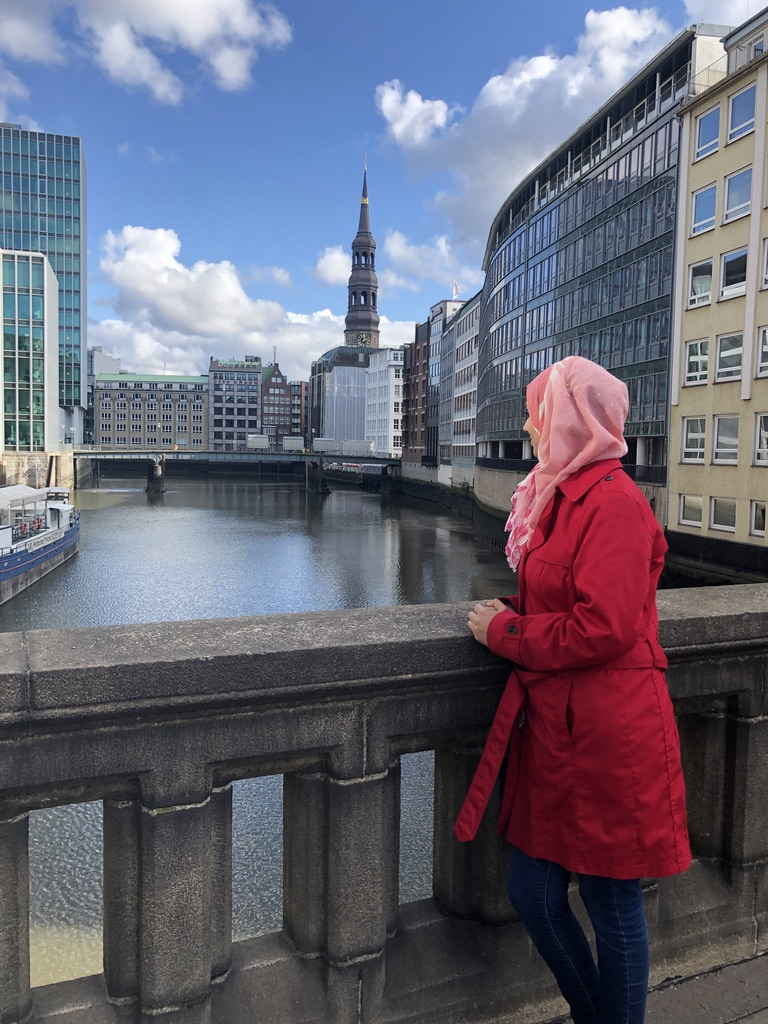
\includegraphics[width=0.7\linewidth]{chapters/chapter2/FigureCh2/img2}
	\caption[fig3short]{fig3Long}
	\label{fig:img3}
\end{wrapfigure}

\lipsum[1-5]

We are going to use this section to put some text in our document and at some points, we are going to inset a reference. This, for example, is going to turn into a reference~\cite{Control-CDW-Okamoto-1992}. This~\cite{Lattice-Dynamics-Fehske-2000} is yet another reference. And so on~\cite{Dynamical-Monkowsky-2017}.

And the gravity waves stuff would come here~\cite{Gravity-Wave-2015}
